\documentclass[../main.tex]{subfiles}

\begin{document}
    % Obwohl andere Sektionen die Softwarearchitektur beschreiben, will man manchmal ein paar wichtige oder komplexe Implementationsdetails erläutern.
    % Dafür ist diese Sektion gedacht. Die Beschreibung der Details soll kurz und knapp gehalten werden.
    % Lieber ein paar Minuten ein-setzen um ein vereinfachtes Ablauf oder Sequenzdiagramm zu zeichnen anstelle von aufwändige Beschreibungen. Beispiele:
    %   •Kurzbeschreibung eines in House Framework
    %   •Data-Binding Ansatz
    %   •Wichtige Elemente des Domänen-Models
    %   •Konfigurationsmechanismus
    %   •Exception-Handling und Logging-Ansatz
    %   •etc.
    % Dies ist ein optionales Kapitel, das nur verwendet wird, wenn notwendig. Bei komplexeren Systeme jedoch sehr häufig der Fall.

	\section{Codebase}
	\par In diesem Kapitel werden allfällige Codestrukturen näher erläutert, sofern diese Erklärungsbedarf besitzen. Ebenfalls aufgeführt werden alle selbstkonzipierten, verwendeten Interfaces.
	
	\subsection{Koordinatensystem}
	\par Das Koordinatensystem benutzt drei Achsen (cube), um ein hexagonales Raster im zweidimensionalen Raum abzubilden. Hexagonale Raster lassen sich auch mit zwei Achsen beschreiben (axial), wobei es in solch einem Fall nötig ist, jede zweite Reihe durch einen Offset zu verschieben. Die axialen lassen sich in kubische Werte umrechnen und umgekehrt. Die kubischen Koordinaten ergeben in ihrer Summe stets 0.
	\par Die jeweiligen Rasterkoordinaten lassen sich durch geschickte Verknüpfung von kubischen und axialen Koordinaten in tatsächliche Raumkoordinaten umrechnen.
	\par Die Implementation richtet sich im Allgemeinen nach der sehr ausführlich beschriebenen \href{https://www.redblobgames.com/grids/hexagons/}{Dokumentation} über hexagonale Raster, die man bei Red Blob Games finden kann.
	\begin{figure}[H]
		\centering
		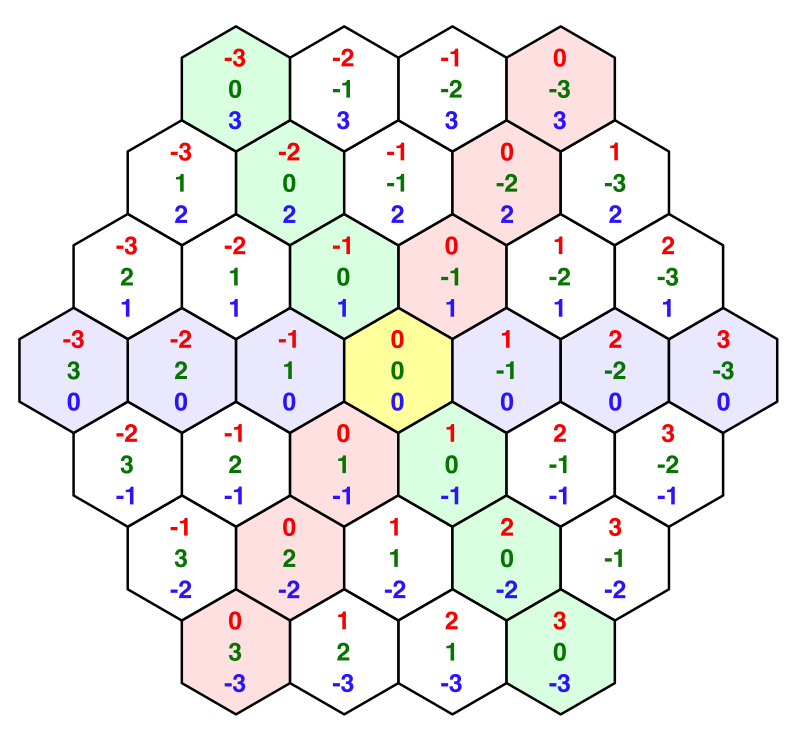
\includegraphics[angle=0, width=0.6\linewidth]{coordinate-system.png}
	\end{figure}

	\subsection{Data-Binding und Event-Handling}
	\begin{figure}[H]
		\centering
		\includegraphics[angle=0, width=0.6\linewidth]{DataBinding_Eventhandling.jpg}
	\end{figure}
	\subsubsection{Data-Binding}
	\par Das Data-Binding wird mittels Kappselung realisiert. Klassen aus der Unity-Umgebung (MonoBehaviours) verwenden Properties, deren Getter-Methoden auf die entsprechenden Interfaces der gekappselten Klassen aus der regulären C\#-Umgebung zurückgreifen. Die Interfaces wiederum wurden von den Logikklassen implementiert und besitzen die gewünschten Daten. Näheres zur Architektur ist im Kapitel \nameref{section:UnityCodeArchitektur} beschrieben.
	\par Damit Daten stets aktuell sind und korrekt repräsentiert werden, wird ein Publish-Subscribe-Pattern verwendet.
	
	\subsubsection{Event-Handling}
	\par Ändern sich Werte auf der C\#-Ebene, so lösen die jeweiligen Klassen einen Event aus, ähnlich dem \href{https://docs.microsoft.com/en-us/dotnet/api/system.componentmodel.inotifypropertychanged?view=net-5.0}{INotifyPropertyChanged}-Interface. MonoBehaviour-Klassen können über die Interfaces an den jeweiligen Events als Subscriber teilnehmen.
	\par Event-Handling auf Unity-Ebene wird durch die Engine selbst bereits abgewickelt. Die Entwickler können sich an den bestehenden Konzepten von \gls{unity} bedienen.
	
	\subsection{Interfaces}
	\label{section:Interfaces}
	\subsubsection{Plättchen / Tile}
	\begin{lstlisting}
  public interface ITile
  {
	#region Events
	event Action TileChangedEvent;
	event Action<Coordinate> RemovalRequestedEvent;
	#endregion
	#region Data
	Coordinate Coordinate { get; set; }
	int Rotation { get; }
	EState State { get; set; }
	ITileType Type { get; set; }
	ITileBehaviour Behaviour { get; set; }
	ITileNature Nature { get; set; }
	#endregion
	#region Logic
	void RequestRemoval();
	void Rotate(int rotation);
	#endregion
  }
	\end{lstlisting}

	\subsubsection{Plättchentyp / TileType}
	\begin{lstlisting}
  public interface ITileType : IFunctionalValues
  {
	EType Type { get; }
	int ValueOfRelationshipTo(EType otherType);
  }
	\end{lstlisting}

	\subsubsection{Plättchenverhalten / TileBehaviour}
	\begin{lstlisting}
  public interface ITileBehaviour : IFunctionalValues
  {
	EBehaviour Behaviour { get; }
	void ApplyBehaviour(ITile originalTile, ITile otherTile);
  }
	\end{lstlisting}

	\subsubsection{Plättchenart / TileNature}
	\begin{lstlisting}
  public interface ITileNature : IFunctionalValues
  {
	ENature Nature { get; }
	IEnumerable<Coordinate> RelevantCoordinates
		(Coordinate coordinate, int rotation);
  }
	\end{lstlisting}

	\subsubsection{Plättchenstapel / TileStack}
	\begin{lstlisting}
  public interface ITileStack
  {
	void InitializeStack();
	void PushTiles(List<ITile> tiles);
	void Push(ITile newTile);
	ITile Pop();
	int Count();
	ITile Peek();
	List<ITile> GetFirstTenTiles();
	void AddNewRandomTiles(int amount);
  }
	\end{lstlisting}

	\subsubsection{Spielfeld / TileMap}
	\begin{lstlisting}
  public interface ITileMap<T> where T : class, ITile
  {
	void PlaceTile(T tile, Coordinate coordinate);
	void RemoveTile(Coordinate coordinate);
	T GetTile(Coordinate coordinate);
	bool IsEmpty(Coordinate coordinate);
	event EventHandler<TileMapEventArgs<T>> TilePlaced;
	event EventHandler<TileMapEventArgs<T>> TileRemoved;
  }
	

	\end{lstlisting}
	\begin{lstlisting}
  public class TileMapEventArgs<T> : EventArgs where T : class, ITile
  {
	public TileMapEventArgs(ITileMap<T> tileMap, T tile)
	{
		Map = tileMap;
		Tile = tile;
	}
	
	public ITileMap<T> Map { get; set; }
	public T Tile { get; set; }
  }
	\end{lstlisting}

	\subsubsection{Punktestand / GameScore}
	\begin{lstlisting}
  public interface IGameScore
  {
	int IncreaseScore(int amount);
	int GetCurrentScore();
	int GetNextScoreThreshold();
	int PointsUntilNextThreshold();
  }
	\end{lstlisting}

	\subsubsection{Punkterechner / TileResolver}
	\par Ein TileResolver wird dafür eingesetzt, die Abwicklung der Spielregeln zu handhaben, nachdem ein Plättchen platziert wurde.
	\begin{lstlisting}
  public interface ITileResolver<T> where T : class, ITile
  {
	void ApplyBehaviour(T tile);
	int CalculatePoints(T tile);
  }
	\end{lstlisting}

	\subsubsection{Wahrscheinlichkeitswert / FunctionalValues}
	\par Um eine spielerisch sinnvolle Verteilung der jeweiligen Plättchentypen, -arten und -verhalten zu erreichen, implementieren all diese Klassen das FunctionalValues Interface. Es liefert eine Gewichtung, die im Kontext zur Auswirkung auf das Spiel steht.
	\begin{lstlisting}
  public interface IFunctionalValues
  {
	int CalculateWeight();
  }
	\end{lstlisting}
\end{document}